% Options for packages loaded elsewhere
\PassOptionsToPackage{unicode,linktoc=all}{hyperref}
\PassOptionsToPackage{hyphens}{url}
\PassOptionsToPackage{dvipsnames,svgnames,x11names}{xcolor}
%
\documentclass[
  a4paper,
]{article}
\usepackage{amsmath,amssymb}
\usepackage{iftex}
\ifPDFTeX
  \usepackage[T1]{fontenc}
  \usepackage[utf8]{inputenc}
  \usepackage{textcomp} % provide euro and other symbols
\else % if luatex or xetex
  \usepackage{unicode-math} % this also loads fontspec
  \defaultfontfeatures{Scale=MatchLowercase}
  \defaultfontfeatures[\rmfamily]{Ligatures=TeX,Scale=1}
\fi
\usepackage{lmodern}
\ifPDFTeX\else
  % xetex/luatex font selection
\fi
% Use upquote if available, for straight quotes in verbatim environments
\IfFileExists{upquote.sty}{\usepackage{upquote}}{}
\IfFileExists{microtype.sty}{% use microtype if available
  \usepackage[]{microtype}
  \UseMicrotypeSet[protrusion]{basicmath} % disable protrusion for tt fonts
}{}
\makeatletter
\@ifundefined{KOMAClassName}{% if non-KOMA class
  \IfFileExists{parskip.sty}{%
    \usepackage{parskip}
  }{% else
    \setlength{\parindent}{0pt}
    \setlength{\parskip}{6pt plus 2pt minus 1pt}}
}{% if KOMA class
  \KOMAoptions{parskip=half}}
\makeatother
\usepackage{xcolor}
\usepackage[margin=25mm]{geometry}
\usepackage{longtable,booktabs,array}
\usepackage{calc} % for calculating minipage widths
% Correct order of tables after \paragraph or \subparagraph
\usepackage{etoolbox}
\makeatletter
\patchcmd\longtable{\par}{\if@noskipsec\mbox{}\fi\par}{}{}
\makeatother
% Allow footnotes in longtable head/foot
\IfFileExists{footnotehyper.sty}{\usepackage{footnotehyper}}{\usepackage{footnote}}
\makesavenoteenv{longtable}
\usepackage{graphicx}
\makeatletter
\def\maxwidth{\ifdim\Gin@nat@width>\linewidth\linewidth\else\Gin@nat@width\fi}
\def\maxheight{\ifdim\Gin@nat@height>\textheight\textheight\else\Gin@nat@height\fi}
\makeatother
% Scale images if necessary, so that they will not overflow the page
% margins by default, and it is still possible to overwrite the defaults
% using explicit options in \includegraphics[width, height, ...]{}
\setkeys{Gin}{width=\maxwidth,height=\maxheight,keepaspectratio}
% Set default figure placement to htbp
\makeatletter
\def\fps@figure{htbp}
\makeatother
\usepackage{svg}
\setlength{\emergencystretch}{3em} % prevent overfull lines
\providecommand{\tightlist}{%
  \setlength{\itemsep}{0pt}\setlength{\parskip}{0pt}}
\setcounter{secnumdepth}{-\maxdimen} % remove section numbering
% definitions for citeproc citations
\NewDocumentCommand\citeproctext{}{}
\NewDocumentCommand\citeproc{mm}{%
  \begingroup\def\citeproctext{#2}\cite{#1}\endgroup}
\makeatletter
 % allow citations to break across lines
 \let\@cite@ofmt\@firstofone
 % avoid brackets around text for \cite:
 \def\@biblabel#1{}
 \def\@cite#1#2{{#1\if@tempswa , #2\fi}}
\makeatother
\newlength{\cslhangindent}
\setlength{\cslhangindent}{1.5em}
\newlength{\csllabelwidth}
\setlength{\csllabelwidth}{3em}
\newenvironment{CSLReferences}[2] % #1 hanging-indent, #2 entry-spacing
 {\begin{list}{}{%
  \setlength{\itemindent}{0pt}
  \setlength{\leftmargin}{0pt}
  \setlength{\parsep}{0pt}
  % turn on hanging indent if param 1 is 1
  \ifodd #1
   \setlength{\leftmargin}{\cslhangindent}
   \setlength{\itemindent}{-1\cslhangindent}
  \fi
  % set entry spacing
  \setlength{\itemsep}{#2\baselineskip}}}
 {\end{list}}
\usepackage{calc}
\newcommand{\CSLBlock}[1]{\hfill\break\parbox[t]{\linewidth}{\strut\ignorespaces#1\strut}}
\newcommand{\CSLLeftMargin}[1]{\parbox[t]{\csllabelwidth}{\strut#1\strut}}
\newcommand{\CSLRightInline}[1]{\parbox[t]{\linewidth - \csllabelwidth}{\strut#1\strut}}
\newcommand{\CSLIndent}[1]{\hspace{\cslhangindent}#1}
\ifLuaTeX
\usepackage[bidi=basic]{babel}
\else
\usepackage[bidi=default]{babel}
\fi
\babelprovide[main,import]{british}
% get rid of language-specific shorthands (see #6817):
\let\LanguageShortHands\languageshorthands
\def\languageshorthands#1{}
% $HOME/.pandoc/defaults/latex-header-includes.tex
% Common header includes for both lualatex and xelatex engines.
%
% Preliminaries
%
% \PassOptionsToPackage{rgb,dvipsnames,svgnames}{xcolor}
% \PassOptionsToPackage{main=british}{babel}
\PassOptionsToPackage{english}{selnolig}
\AtBeginEnvironment{quote}{\small}
\AtBeginEnvironment{quotation}{\small}
\AtBeginEnvironment{longtable}{\centering}
%
% Packages that are useful to include
%
\usepackage{graphicx}
\usepackage{subcaption}
\usepackage[inkscapeversion=1]{svg}
\usepackage[defaultlines=4,all]{nowidow}
\usepackage{etoolbox}
\usepackage{fontsize}
\usepackage{newunicodechar}
\usepackage{pdflscape}
\usepackage{fnpct}
\usepackage{parskip}
  \setlength{\parindent}{0pt}
\usepackage[style=american]{csquotes}
% \usepackage{setspace} Use the <fontname-plus.tex> files for setspace
%
\usepackage{hyperref} % cleveref must come AFTER hyperref
\usepackage[capitalize,noabbrev]{cleveref} % Must come after hyperref
\let\longdivision\relax
\usepackage{longdivision}
% noto-plus.tex
% Font-setting header file for use with Pandoc Markdown
% to generate PDF via LuaLaTeX.
% The main font is Noto Serif.
% Other main fonts are also available in appropriately named file.
\usepackage{fontspec}
\usepackage{setspace}
\setstretch{1.3}
%
\defaultfontfeatures{Ligatures=TeX,Scale=MatchLowercase,Renderer=Node} % at the start always
%
% For English
% See also https://tex.stackexchange.com/questions/574047/lualatex-amsthm-polyglossia-charissil-error
% We use Node as Renderer for the Latin Font and Greek Font and HarfBuzz as renderer ofr Indic fonts.
%
\babelfont{rm}[Script=Latin,Scale=1]{NotoSerif}% Config is at $HOME/texmf/tex/latex/NotoSerif.fontspec
\babelfont{sf}[Script=Latin]{SourceSansPro}% Config is at $HOME/texmf/tex/latex/SourceSansPro.fontspec
\babelfont{tt}[Script=Latin]{FiraMono}% Config is at $HOME/texmf/tex/latex/FiraMono.fontspec
%
% Sanskrit, Tamil, and Greek fonts
%
\babelprovide[import, onchar=ids fonts]{sanskrit}
\babelprovide[import, onchar=ids fonts]{tamil}
\babelprovide[import, onchar=ids fonts]{greek}
%
\babelfont[sanskrit]{rm}[Scale=1.1,Renderer=HarfBuzz,Script=Devanagari]{NotoSerifDevanagari}
\babelfont[sanskrit]{sf}[Scale=1.1,Renderer=HarfBuzz,Script=Devanagari]{NotoSansDevanagari}
\babelfont[tamil]{rm}[Renderer=HarfBuzz,Script=Tamil]{NotoSerifTamil}
\babelfont[tamil]{sf}[Renderer=HarfBuzz,Script=Tamil]{NotoSansTamil}
\babelfont[greek]{rm}[Script=Greek]{GentiumBookPlus}
%
% Math font
%
\usepackage{unicode-math} % seems not to hurt % fallabck
\setmathfont[bold-style=TeX]{STIX Two Math}
\usepackage{amsmath}
\usepackage{esdiff} % for derivative symbols
% \renewcommand{\mathbf}{\symbf}
%
%
% Other fonts
%
\newfontfamily{\emojifont}{Symbola}
%

\usepackage{titling}
\usepackage{fancyhdr}
    \pagestyle{fancy}
    \fancyhead{}
    \fancyfoot{}
    \renewcommand{\headrulewidth}{0.2pt}
    \renewcommand{\footrulewidth}{0.2pt}
    \fancyhead[LO,RE]{\scshape\thetitle}
    \fancyfoot[CO,CE]{\footnotesize Copyright © 2006\textendash\the\year, R (Chandra) Chandrasekhar}
    \fancyfoot[RE,RO]{\thepage}
%
\usepackage{newunicodechar}
\newunicodechar{√}{\textsf{√}}
\ifLuaTeX
  \usepackage{selnolig}  % disable illegal ligatures
\fi
\usepackage{bookmark}
\IfFileExists{xurl.sty}{\usepackage{xurl}}{} % add URL line breaks if available
\urlstyle{sf}
\hypersetup{
  pdftitle={From Calculus to Analysis: Limits},
  pdfauthor={R (Chandra) Chandrasekhar},
  pdflang={en-GB},
  colorlinks=true,
  linkcolor={DarkOliveGreen},
  filecolor={Purple},
  citecolor={DarkKhaki},
  urlcolor={Maroon},
  pdfcreator={LaTeX via pandoc}}

\title{From Calculus to Analysis: Limits}
\author{R (Chandra) Chandrasekhar}
\date{2024-03-24 | 2024-05-21}

\begin{document}
\maketitle

\thispagestyle{empty}


\begin{flushright}

\begin{footnotesize}

The fundamental concept on which the whole of mathematical\\
analysis ultimately rests is that of the limit of an infinite sequence
\(a_{n}\).

\textsc{Richard Courant and Fritz John}\\
\emph{Introduction to Calculus and Analysis}, Volume I, p 60.

\end{footnotesize}

\end{flushright}

\begin{quote}
This is the first of several blogs that are devoted to the transition
from calculus to analysis. The focus in this blog is the concept of
limits, as applied to an infinite real sequence.

Parts of this blog have been lifted from the chapter entitled
``Mathematics at University'' from my book,
\href{https://swanlotus.netlify.app/sas}{\emph{Secrets of Academic
Success}}, which is
\href{https://swanlotus.netlify.app/sas-manuscript/SAS-partial.pdf}{available
as a free PDF download}. However, since that chapter was written, I have
myself gained greater understanding on why calculus at high school
needed to morph into analysis at university. Accordingly, the material
has been augmented, but kept simple enough to be accessible to a high
school student just entering university.

I am not a professional mathematician, and make no claim to rigour in
this blog. Rather, I hope to demystify analysis from the grip of symbols
by explaining its
\href{https://www.thefreedictionary.com/raison+d+etre}{\emph{raison
d'être}} in plain English. In the process, I hope analysis appears less
forbidding and more friendly.
\end{quote}

\subsection{The transition from high school to
university}\label{the-transition-from-high-school-to-university}

At high school you were taught how to integrate and differentiate. You
were exposed to all sorts of tricks and special techniques---such as the
chain rule for differentiation, and integration by parts for
integration. If you revelled in mastering and applying such techniques,
you might find that what succeeds high school \emph{calculus}, is a
\href{https://www.dictionary.com/browse/a-horse-of-a-different-color}{horse
of an entirely different colour}, called \emph{analysis}, at university.

You might even be alarmed that rather than having to solve routine
problems for the value of some quantity, or simply to work through and
demonstrate a fact in a straightforward fashion, you are now required to
\emph{prove} theorems: something that requires a different mindset and
skill set.

\subsection{Why the change?}\label{why-the-change}

High school calculus appeals to intuition and the visual sense, through
\emph{geometric} ideas like slopes and areas. Words like ``approaches'',
``tends to'', etc., signify motion and resonate with our sense of space
and time.

Analysis, on the other hand, is logically precise and uses
\emph{arithmetic} as the basis for deriving results. Intuition has given
way to logical precision, and pictures have yielded to symbols. The
implicit scaffolding of familiar ideas like space and time---borrowed
from our everyday experience---has been replaced with the clinical
precision of inequalities and
\href{https://math.libretexts.org/Bookshelves/Mathematical_Logic_and_Proof/Book\%3A_Mathematical_Reasoning__Writing_and_Proof_(Sundstrom)/02\%3A_Logical_Reasoning/2.04\%3A_Quantifiers_and_Negations}{universal
and existential quantifiers}.

The logically indefensible infinitesimals of calculus have given way to
the rigorously justifiable limits and infinite sums of analysis. Numbers
alone provide the foundation, and this required the idea of a number
itself to be strengthened as an abstraction beyond question or doubt.

All this takes some getting used to. We have moved from an innocent
nature-hewn cave to a fabricated apartment block that reaches for the
sky. Questions such as, ``Is this change really necessary?'' and ``If it
ain't broke, why fix it?'' arise in consequence.

But the sober truth is that high school calculus \emph{is} ``broke''. It
is fun-filled, but nevertheless, a convenient fiction by mathematical
standards. Two centuries passed between the discovery of the calculus as
a magical computing machine, and the recognition of the need to fix it
so that it would work robustly in all circumstances.

In this sense, the progression from calculus to analysis is similar to
the accretion of zero and the negative numbers to the natural numbers,
or the introduction of imaginary numbers to account for roots of certain
polynomials. All such changes were resisted at first, just like a new
pair of shoes that initially pinch, but time and usage have borne
testament to the wisdom behind the change. The somewhat painful
transition from calculus to analysis will prove to be the same.

\subsection{Geometry's fall from
favour}\label{geometrys-fall-from-favour}

Mathematics texts at high school level are generously and often
colorfully illustrated, especially when dealing with geometry. But, if
you look at any university-level analysis textbook, colour would have
taken heel, and pictures will be the exception rather than the rule. For
those who think in pictures, this will come as a letdown, accompanied by
the puzzling question, ``Why?''

Geometric intuition, upon which Greek mathematics rested securely for
well nigh two centuries, was not infallible. The development of new
\href{https://en.wikipedia.org/wiki/Non-Euclidean_geometry}{non-Euclidean
geometries} in the nineteenth century robbed mathematics of its innocent
certitude in geometric foundations. And the resulting revolution, called
the \href{https://en.wikipedia.org/wiki/Erlangen_program}{Erlangen
program}, made algebra the basis of classifying geometry itself.

Our everyday experience is rooted in our sense of space and time. So, I
will attempt to illustrate the ideas of analysis using pictures wherever
I can, so that the alien syntax and symbology of analysis is buttressed
by the reassuring presence of equivalent pictures. Unfortunately, many
introductory analysis books are illustrated scantily, if at all.

\subsection{Holes in the real number
line}\label{holes-in-the-real-number-line}

What do irrational numbers have to do with analysis? Quite a lot,
really.

Real analysis lives on the real number line. From the time of the
Pythagoreans, the irrational numbers have caused mathematicians' hearts
to skip a beat. ``Are irrational numbers really numbers? If so, where do
they live?'' The absence of irrational numbers meant that there were
holes in the real number line.

The Greeks circumvented this by limiting the irrational numbers to
geometric contexts. The ratio of the circumference of a unit circle to
its diameter is \(\pi\). The diagonal of a unit square is \(\sqrt{2}\).
``Let them live geometrically as \emph{lengths}, but let us remain
silent about their existence elsewhere.'' It was a dichotomy between
\emph{counting} and \emph{measurement} or between the \emph{discrete}
and the \emph{continuous}.

Even today, the sets for the \emph{natural numbers}, the
\emph{integers}, the \emph{rational numbers} all have their own
symbols---\(\mathbb{N}\), \(\mathbb{Z}\), \(\mathbb{Q}\), respectively,
but not the irrational numbers. That should be clue enough to indicate
that the irrationals were more than a handful for mathematicians to
contend with, especially if they were doubts about where they rightfully
belonged.

The rational numbers, when expressed as decimals, either have a
\emph{finite} decimal representation, like
\(\frac{1}{2} = 0.5\)\footnote{To muddy matters even more,
  \(\frac{1}{2} = 0.4999\dots\) is an equally a valid representation!},
or an \emph{infinitely recurring} decimal representation like
\(\frac{1}{3} = 0.333\dots\).

The irrational number \(\sqrt{2}\)---when expressed as a
decimal---neither terminates nor recurs without end. Its unpredictable
digits go on and on and on. So, where exactly does \(\sqrt{2}\) sit on
the real line?

This troubling question went unanswered until
\href{https://plato.stanford.edu/entries/dedekind-foundations/}{Richard
Dedekind} skilfully introduced the
\href{https://www.britannica.com/science/Dedekind-cut}{Dedekind cut} to
legitimately accommodate the irrationals as first-class citizens of the
real number line, fully capable of undergoing all the arithmetic
operations of the rational numbers\footnote{Cauchy gave an alternative
  justification---to accommodate the rationals into the reals---via the
  \hyperref[cauchy-sequence]{sequence that bears his name}}.

The inclusion of the irrational numbers into the fold of real numbers
along with the rational numbers \(\mathbb{Q}\),
\href{https://en.wikipedia.org/wiki/Completeness_of_the_real_numbers}{completes}
the set of real numbers, \(\mathbb{R}\). Strengthening the foundations
of the real numbers was a prerequisite to the introduction of rigour in
analysis. There are no more holes in the real line.

Numbers such as \(\pi\) and \(\sqrt{2}\) arising from the simplest plane
geometry can now be accommodated legitimately as first-class citizens of
the real number line.

\subsection{Approximating an
irrational}\label{approximating-an-irrational}

When we use a calculator to key in \(\sqrt{2}\), we see a sequence of
digits on the display. But that sequence is only an
\emph{approximation}. \emph{The exact decimal representation of an
irrational number does not exist}. So, when we calculate or compute with
irrationals, we are using \emph{rational approximations} in their stead.
And for real world purposes, that approximation suffices.

A real sequence \(S(n)\), also written as \((a_{n})\), is a function
from the set of natural numbers to the set of real numbers.
Symbolically, this is stated as \(S: \mathbb{N} \to \mathbb{R}\), and as
\(n \mapsto a_{n}\).

My calculator gives me the following approximation for \(\sqrt{2}\):
\(1.414213562\dots\). Suppose we form the sequence \[
S = (a_n) = 1, 1.4, 1.41, 1.414, 1.4142, 1.41421, 1.414213, 1.4142135, 1.41421356, 1.414213562 \dots
\] obtained by \emph{truncating} the decimal representation, with
\(a_{1} = 1\), \(a_{2} = 1.4\), until \(a_{9} = 1.41421356\). Note that
\(S\) is an \emph{infinite}, real sequence. The successive terms in the
sequence are successive rational approximations to the value
\(\sqrt{2}\)---each more accurate than the previous one---but with the
proviso that there is \emph{no exact decimal representation} for the
value of \(\sqrt{2}\), except via the \emph{symbol} itself.

Note the following points:

\begin{enumerate}
\item
  The sequence \(S\) goes on without end.
\item
  The sequence \(S\) has been constructed, one digit at a time, to
  approximate the value of \(\sqrt{2}\). Its terms therefore represent
  \emph{rational approximations} to \(\sqrt{2}\).
\item
  We may assert---by virtue of the construction of \(S\)---that a later
  term in the sequence is a more accurate approximation to \(\sqrt{2}\)
  than an earlier term. The sequence
  \href{https://en.wikipedia.org/wiki/Convergent_series}{converges} to
  \(\sqrt{2}\).
\item
  \(a_{n}\) inexorably \emph{tends to} the value \(\sqrt{2}\), as we
  keep on adding successive terms to the sequence.
\item
  Because \(a_{n}\) can never equal \(\sqrt{2}\), we \emph{cannot
  equate} \(a_{n}\) to \(\sqrt{2}\) for any \emph{finite}
  \(n \in \mathbb{N}\).
\item
  The \href{https://en.wikipedia.org/wiki/Limit_(mathematics)}{limit} in
  this case, \(\sqrt{2}\), is therefore \emph{not} a member of the
  sequence.
\end{enumerate}

In symbols, we write
\(a_{n} \to \sqrt{2} \text{ as } n \to \infty\).\footnote{Infinity is
  not a natural number.} Alternatively, we may write \[
\lim_{n \to \infty}a_{n} = \sqrt{2}.
\] But the equality sign here pertains to an \emph{infinite process} and
cannot be treated in the same cavalier way as we would the garden
variety equality sign in \(2 + 3 = 5\).

But this symbology is imprecise because we are handwaving with the words
``tends to'' indicated by \(\to\) and ``infinity'' indicated by
\(\infty\). We will re-visit the issue of how to make precise and
watertight the idea of a limit when we shed intuitive notions like
``tends to'' and ``infinity'' and replace it with a strict arithmetical
criterion.

\subsection{Ordered Archimedean field}\label{ordered-archimedean-field}

Two properties of real numbers are highlighted as being essential for
real analysis:

\begin{enumerate}
\def\labelenumi{\alph{enumi}.}
\item
  The \href{https://en.wikipedia.org/wiki/Law_of_trichotomy}{trichotomy}
  of the real numbers, which states that every real number is either
  positive, zero, or negative. Given any two real numbers, \(x\) and
  \(y\), \emph{only one} of the following three statements is true:
  \(x < y\), or \(x = y\), or \(x > y\).
\item
  The \href{https://planetmath.org/archimedeanproperty}{Archimedean
  property} which forbids
  \href{https://en.wikipedia.org/wiki/Infinity}{infinities}\footnote{Which
    may be colloquially stated as there is no largest natural number.}
  and \href{https://en.wikipedia.org/wiki/Infinitesimal}{infinitesimals}
  from being real numbers. It states that:

  \begin{enumerate}
  \def\labelenumii{(\roman{enumii})}
  \tightlist
  \item
    For \emph{any} real number \(x\), there is a natural number \(n\)
    such that \(n > x\).\footnote{\(\forall x \in \mathbb{R}, \exists n \in \mathbb{N} \text{ such that } n > x.\)}
  \item
    For \emph{any positive} real number \(y\), there is a natural number
    \(n\) such that \(\frac{1}{n} < y\).\footnote{\(\forall y \in \mathbb{R}, y > 0, \exists n \in \mathbb{N} \text{ such that } \frac{1}{n} < y\).}
  \end{enumerate}
\end{enumerate}

\subsection{Inequalities and
distances}\label{inequalities-and-distances}

Calculus problems are generally concerned with \emph{evaluating} some
quantity and are therefore centred around \emph{equalities}.

Analysis, on the other hand, relies heavily on logical statements about
quantities whose exact values may not be known, but about whom
statements of \emph{relative size} need to be made. This is where
\emph{inequalities} enter the discourse.\footnote{You would have already
  seen from above how inequalities are used to define an Archimedean
  field.}

This change in emphasis can be disconcerting. Students seeking to
familiarize themselves with manipulations of inequalities should consult
entry-level texts dealing with this subject
{[}\citeproc{ref-kazarinoff-1961}{1}--\citeproc{ref-alsina-nelsen-2009}{3}{]}.

When the derivative\footnote{To be covered in a later blog.} was defined
geometrically, in high school, as the value of the slope of a tangent to
the graph of the function at a particular point, the geometrical
relationship alone sufficed to encapsulate the definition and to help
compute the value.

However, when the derivative is defined as a
\href{https://en.wikipedia.org/wiki/Limit_(mathematics)}{\emph{limit}},
using arithmetic instead of geometry, we do not have \emph{intuitive}
markers to guide us. And while such markers are serviceable, they are
not infallible. Therefore, we need some symbols and operations to
contend with ideas like the ``closeness'' of two points, etc.

This is where we encounter two mathematical devices quintessential to
analysis and much of modern mathematics:

\begin{enumerate}
\def\labelenumi{\alph{enumi}.}
\item
  Inequalities: by understanding and manipulating the symbols \(>\) and
  \(<\), we can work toward watertight definitions that serve to
  constrain what we are talking about.
\item
  Distance: by using a sensible definition of the distance between two
  points, we may measure their ``closeness''. Geometry and intuition
  would then have been replaced by arithmetic and precision.

  If there are two \emph{distinct} real numbers \(p\) and \(q\),
  \(|p - q|\) defines the positive number that quantifies their
  separation or distance. Since we are on the real line, the
  \href{https://mathworld.wolfram.com/AbsoluteValue.html}{\emph{absolute
  value function}} is used for this purpose. See \cref{fig:absolute} for
  the graph of \(y = |x]\).

  \begin{figure}
  \centering
  \includesvg[width=0.8\textwidth,height=\textheight]{images/absolute-value.svg}
  \caption{The non-negative, absolute value function, \(y = |x|\), which
  is the distance function on the real line.}\label{fig:absolute}
  \end{figure}

  The ``arbitrarily close'' condition of calculus may then be couched
  more precisely thus:

  For arbitrary
  \(\varepsilon > 0 \dots | p - q | < \varepsilon\)\footnote{The
    arbitrariness is still there via \(\varepsilon\) but the closeness
    has been strictly quantified by the distance function and the
    enquality.}.
\end{enumerate}

This incantation will become so familiar that it will become
unremarkable when you devote time and practice to analysis. And notice
the usefulness of inequalities here.

\subsection{\texorpdfstring{Approximation for \(\sqrt{2}\)
revisited}{Approximation for \textbackslash sqrt\{2\} revisited}}\label{approximation-for-sqrt2-revisited}

We now have a quantitative description for a measure of closeness. Let
us put it to use in the example from
\hyperref[approximating-an-irrational]{Approximating an irrational}
above. We know that our approximation becomes better as \(n\) increases.

Let us \emph{fix the admissible error} to be some positive real number
\(\varepsilon\). This means that the error is never zero: which is as it
should be. We may then say that as long as \(n\) is larger than some
number, say \(m\), the error or difference between between \(a_{n}\) and
\(\sqrt{2}\) will be less than \(\varepsilon\).

To express this with few words and many symbols, we take recourse to two
ideas from logic:

\begin{enumerate}
\def\labelenumi{\alph{enumi}.}
\item
  The
  \href{https://en.wikipedia.org/wiki/Universal_quantification}{universal
  quantifier}, \(\forall\), which is spoken as ``for all'', ``for any'',
  or ``given any''.
\item
  The
  \href{https://en.wikipedia.org/wiki/Existential_quantification}{existential
  quantifier}, \(\exists\), which is spoken, as ``there exists'',
  ``there is at least one'', or ``for some''.
\end{enumerate}

Strangely, these symbols generalize rather than particularize. So, how
do they tighten up and make more precise those statements whose truth we
wish to establish? Along with inequalities, how do they help make
precise the notions that were handwaved away in calculus?

We may now precisely state:
\begin{equation}\phantomsection\label{eq:epsilon}{
\forall \varepsilon > 0, \exists m \in \mathbb{N} \text{ such that } n > m \implies |a_{n} - \sqrt{2}| < \varepsilon.
}\end{equation}

In plain English, this reads: ``For all values of the
\href{https://mathworld.wolfram.com/Epsilon.html}{Greek letter epsilon,
\(\varepsilon\)}, greater than zero, there exists a natural number \(m\)
such that whenever the natural number \(n\) is greater than \(m\), the
distance between the \(n^{\textrm{th}}\)\textsuperscript{th} term of the
sequence, \(a_{n}\), and the square root of two, \(\sqrt{2}\), is less
than epsilon.''

This definition of a limit starts out with the error variable
\(\varepsilon\) rather than with the index \(m\), above which the
specified error is not exceeded. This may appear counter-intuitive, but
if you think of it like a shepherd does, you would want to corral your
flock before counting it.

The following points are noteworthy:

\begin{enumerate}
\item
  Apart from the limit, which in our case is \(\sqrt{2}\), there is no
  other particular value used in the definition.
\item
  We use the inequality \(|a_{n} - \sqrt{2}| < \varepsilon\) because no
  term of \(S\) actually equals \(\sqrt{2}\).
\item
  By being silent on the value of \(\varepsilon\), except to require it
  to be positive, we may squeeze the error to as small as we want, and
  still not run afoul of any constraints regarding non-equality of any
  \(a_{n}\) with \(\sqrt{2}\). This formulation neatly encapsulates the
  notion of ``tends to, or approaches, but does not equal'', with a
  distance measure that may be made arbitrarily small, but not equal
  zero.\footnote{In hindsight, analysis started off as tidying up the
    loose ends of calculus, but ended up strengthening the whole edifice
    of mathematics, as its very foundations were impacted.}
\item
  The need for \(\mathbb{R}\) to be an
  \hyperref[ordered-archimedean-field]{Ordered Archimedean field} is
  apparent here. We have arbitrarily small numbers, but no
  infinitesimals, and there is no upper bound on the natural numbers.
\end{enumerate}

A pictorial illustration is given in \cref{fig:nested} of what is
happening on the real number line as we progressively approximate
\(\sqrt{2}\).

\begin{figure}
\centering
\includesvg[width=0.9\textwidth,height=\textheight]{images/nested-intervals.svg}
\caption{Nested sequences \([a_i, L]\) vis-a-vis the limit \(L\), which
represents \(\sqrt{2}\) in this case.}\label{fig:nested}
\end{figure}

Note that this figure is not to scale and is not of the actual values
given in \hyperref[approximating-an-irrational]{Approximating an
irrational} but is rather an illustration of what happens as successive
approximations become progressively closer to the limit\footnote{The
  figure is purely didactic; if it were literal, the later ticks would
  be overwritten and the later labels would obscure each other.}.

We know the the limit is \(\sqrt{2}\) because we constructed the
sequence so. Moreover, we are not approaching the limit from
\emph{above} but rather only from \emph{below} by using the successive
digits that the calculator spewed out.

The following observations apply to the
\href{https://mathworld.wolfram.com/ClosedInterval.html}{closed
intervals}, \([a_1, L]\), \([a_2, L]\), \([a_3, L]\), \([a_4, L]\):

\begin{enumerate}
\def\labelenumi{\alph{enumi}.}
\item
  \(L\), representing \(\sqrt{2}\), is the \emph{upper bound} of all the
  intervals. We do not exceed \(L\) as we are approaching it from below.
  Note also that we may include \(\sqrt{2}\) as the end point of a
  closed interval in the real line, like \([a_1, \sqrt{2}]\), because
  the irrationals are first-class citizens of the real line.
\item
  As we move from \(a_1\) to \(a_4\), the intervals \([a_i, L]\), keep
  getting smaller.
\item
  The intervals are
  \href{https://en.wikipedia.org/wiki/Nested_intervals}{nested}:
  \([a_1, L] \supset [a_2, L] \supset [a_3, L] \supset [a_4, L]\).
\end{enumerate}

\subsection{Nested sequence of
intervals}\label{nested-sequence-of-intervals}

When a limit is approached from above as well as below---as illustrated
in \cref{fig:nested-bilateral}---there is a nested sequence of
\emph{closed intervals}, \([a_1, b_1]\), \([a_2, b_2]\), \([a_3, b_3]\),
and \([a_4, b_4]\), each of which contains the limit \(L\). Since each
each interval \([a_{i+1}, b_{i+1}]\) is contained in its predecessor,
\([a_{i}, b_{i}]\), the limit \(L\) is contained in the innermost
interval, which also happens to be the \emph{intersection set} of all
the intervals.

\begin{figure}
\centering
\includesvg[width=0.9\textwidth,height=\textheight]{images/nested-bilateral.svg}
\caption{Nested intervals \([a_i, b_i]\) where the limit \(L\) lies
within the innermost interval, and therefore within all
intervals.}\label{fig:nested-bilateral}
\end{figure}

For those seeking a concrete image for this abstract ``nested intervals
on the real line'' idea,
\href{https://en.wikipedia.org/wiki/Matryoshka_doll}{Matryoshka dolls,
or Russian dolls}, are a very serviceable, accurate, and unforgettable
metaphor, as shown in \cref{fig:matryoshka}.

\begin{figure}
\centering
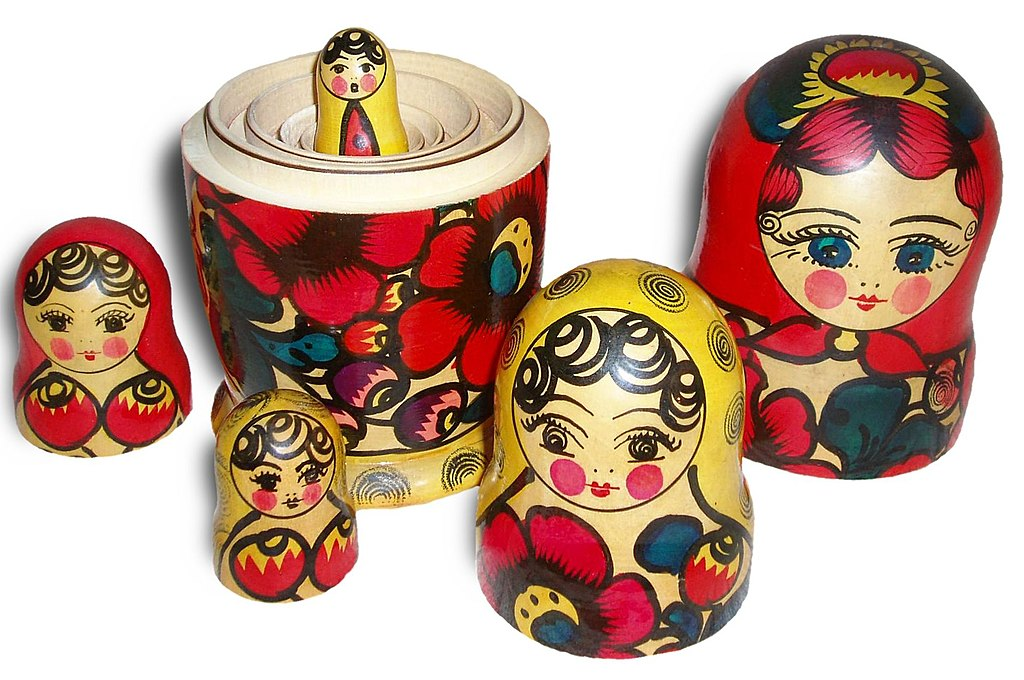
\includegraphics[width=0.8\textwidth,height=\textheight]{images/matryoshka-open.jpg}
\caption[Nested matryoshka dolls, or Russian dolls, serve as a memorable
metaphor for nested intervals.]{Nested matryoshka dolls, or Russian
dolls, serve as a memorable metaphor for nested
intervals.\footnotemark{}}\label{fig:matryoshka}
\end{figure}
\footnotetext{From
  \href{https://upload.wikimedia.org/wikipedia/commons/thumb/d/d2/Russian-Matroshka_no_bg.jpg/1024px-Russian-Matroshka_no_bg.jpg}{Wikimedia}
  by user
  \href{https://commons.wikimedia.org/wiki/User:Fanghong}{Fanghong}
  GFDL.}

\subsection{\texorpdfstring{\href{https://en.wikipedia.org/wiki/Augustin-Louis_Cauchy}{Cauchy}
sequence}{Cauchy sequence}}\label{cauchy-sequence}

A \href{https://en.wikipedia.org/wiki/Cauchy_sequence}{Cauchy sequence}
is a sequence of numbers whose successive terms are spaced apart more
and more closely as the sequence progresses. In symbols, if the sequence
is denoted by \(S = (a_n)\), then for a Cauchy sequence, \[
\forall \varepsilon > 0, \exists N \in \mathbb{N} \text{ such that } n > N \text{ and } m > N \implies |a_n - a_m| < \varepsilon.
\] This ``bunching'' property of later terms in the sequence is
intuitively reassuring, as it is what we would expect when a sequence
converges. It is also a necessary and sufficient condition for a
sequence to converge to a limit.

\subsection{Core texts on analysis}\label{core-texts-on-analysis}

I am aware of three classic two-volume texts that, to me, are remarkably
well-written. The authors of these texts have taken pains to make the
material accessible to students commencing analysis courses. The texts
are:

\begin{enumerate}
\def\labelenumi{\arabic{enumi}.}
\item
  Richard Courant and Fritz John: \emph{Introduction to Calculus and
  Analysis, Volumes I and II}, 1989. This is a classic from a different
  vintage that has stood the test of time. It is more generously
  illustrated than most analysis texts
  {[}\citeproc{ref-courant-john-one}{4},\citeproc{ref-courant-john-two}{5}{]}.
\item
  Terence Tao: \emph{Analysis I} and \emph{Analysis II}, 2022. This text
  was especially written to ease students into analysis. It could have
  as well been called ``Analysis from Scratch''. It is a well-paced,
  student-friendly text, where the author has taken pains to explain
  issues, as if talking to a beginner student.
  {[}\citeproc{ref-tao-one-2022}{6},\citeproc{ref-tao-two-2022}{7}{]}.
\item
  Vladimir A Zorich: \emph{Analysis I} and \emph{Analysis II}, 2015 and
  2016. These are translations of the original texts in Russian. Besides
  rigour, these texts are grounded in actual applications of analysis,
  and should appeal to physicists and engineers as well
  {[}\citeproc{ref-zorich-one-2015}{8},\citeproc{ref-zorich-two-2016}{9}{]}.
\end{enumerate}

You, the student must find out which author's writing resonates best
with you, and use that book as your anchor text. My favourite text on
introductory analysis is Rosenlicht's \emph{Introduction to Analysis}
{[}\citeproc{ref-rosenlicht1986}{10}{]}. It is a marvel of clarity and
is not too expensive to own. Read and work through it if you can.

\begin{figure}
\centering
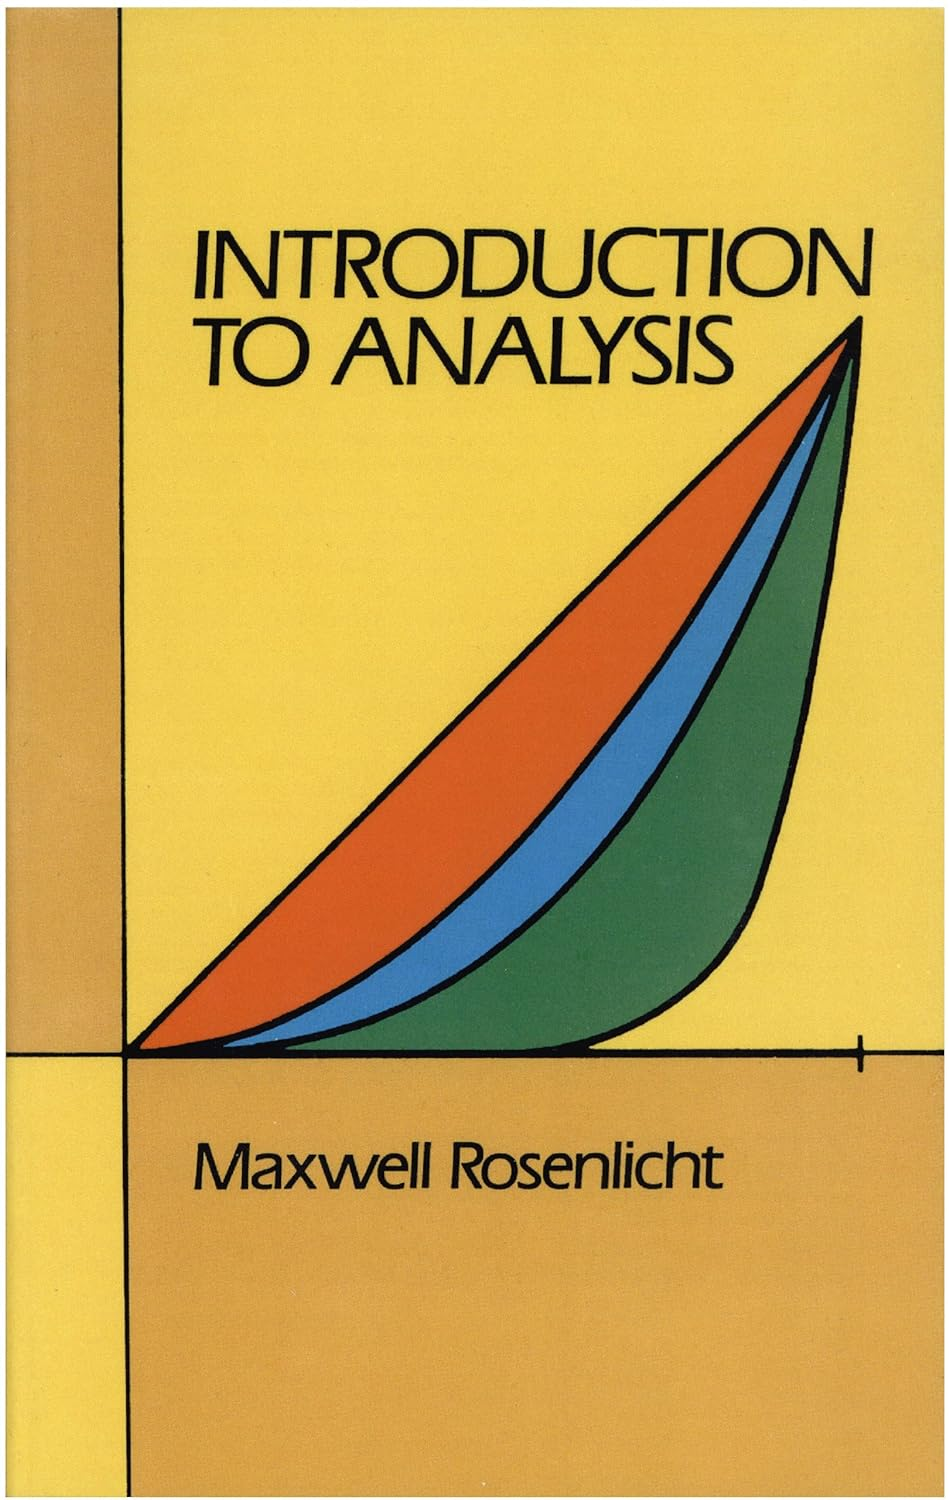
\includegraphics[width=0.4\textwidth,height=\textheight]{images/rosenlicht.jpg}
\caption{Maxwell Rosenlicht's \emph{Introduction to Analysis}, which is
my favourite text on analysis.}\label{fig:rosenlicht}
\end{figure}

\subsection{Other texts on analysis}\label{other-texts-on-analysis}

Besides the core texts I have referred to above, several others have
been written to highlight the differences between calculus and analysis,
and to ease the transition from the one to the other. Their focus and
flavour vary. This list is based on my personal experience and bias:
choose the texts that echo with your own predilections.

A very readable and fascinating recountal of the reasons why analysis
\emph{had to arise} is given in Bressoud's text
{[}\citeproc{ref-bressoud2007}{11}{]} \emph{A Radical Approach to Real
Analysis}. The time spent reading it will be well rewarded with a
quantum jump in your mathematical understanding and maturity.

Gardiner's text \emph{Understanding Infinity: The Mathematics of
Infinite Processes} {[}\citeproc{ref-gardiner2002}{12}{]} is a re-issue
of an earlier book {[}\citeproc{ref-gardiner1982}{13}{]}, that uses
infinite processes as the theme. It is not confined to analysis alone,
but will enlighten the reader familiar with calculus, on \emph{why}
analysis had to arise.

Abbott's book {[}\citeproc{ref-abbott2001}{14}{]} is another text which
gives clear, comprehensible motivations and explanations without losing
rigour.

Two more recent texts that bridge the calculus-analysis divide are those
by Ghorpade and Limaye {[}\citeproc{ref-ghorpadelimaye2006}{15}{]}, and
Brannan {[}\citeproc{ref-brannan2006}{16}{]}. Both of them are very well
written, and have more illustrations than a standard analysis text: they
will find favour with visual learners.

\subsection{Epilogue}\label{epilogue}

There has been a fair bit of huffing and puffing to get to this point.
Has it been worth it?

We have laid a strong foundation for the real numbers by including the
irrationals, circumventing infinitesimals, and defining a limit without
using ideas from time and space, but rather using measures of distance,
and inequalities to denote vanishingly small quantities that,
nevertheless, do not ever equal zero. If you think that this is all
\href{https://www.powerthesaurus.org/much_ado_about_nothing/synonyms}{much
ado about nothing} then, you are unlikely to appreciate analysis any
further.
\href{https://www.spanishdict.com/translate/adios\%20amigo}{Adios
Amigo!}

But if you think that the view from the top was worth the slog of the
climb, you will be better placed to appreciate how differentiation,
integration, and Fourier analysis benefited from the thorough renovation
of the foundations of mathematics that led to analysis. These will be
the subjects of future blogs.

We have considered the limit of a real sequence in this blog. We will
move from the discrete to the continuous, from sequence to function, in
a future blog, and see what that augurs for the concept of a limit. We
will then consider differentiation and integration and try to fathom why
the changed basis offered by analysis for these two pivotal operations
of calculus is the way to go.

A useful metaphor is the renovation of a decrepit house. Renovating
while living in it is tedious and inconvenient. But once the renovation
has been completed, the pleasure of occupying a solidly built near-new
house knows no end. That is how I view the transition from calculus to
analysis.

\subsection{Feedback}\label{feedback}

I am a non-mathematician working outside academia. So, errors are likely
in the exposition. Please
\href{mailto:feedback.swanlotus@gmail.com}{email me} your corrections
and comments please.

\noindent A PDF version of this article is
\href{./from-calculus-to-analysis.pdf}{available for download here}:

\begin{small}

\begin{sffamily}

\url{https://swanlotus.netlify.app/blogs/from-calculus-to-analysis.pdf}

\end{sffamily}

\end{small}

\section*{References}\label{bibliography}
\addcontentsline{toc}{section}{References}

\phantomsection\label{refs}
\begin{CSLReferences}{0}{0}
\bibitem[\citeproctext]{ref-kazarinoff-1961}
\CSLLeftMargin{{[}1{]} }%
\CSLRightInline{Nicholas D Kazarinoff. 1961. \emph{Geometric
inequalities}. The Mathematical Association of America.}

\bibitem[\citeproctext]{ref-beckenbach-bellman-1962}
\CSLLeftMargin{{[}2{]} }%
\CSLRightInline{Edwin Beckenbach and Richard Bellman. 1962. \emph{An
introduction to inequalities}. The Mathematical Association of America.}

\bibitem[\citeproctext]{ref-alsina-nelsen-2009}
\CSLLeftMargin{{[}3{]} }%
\CSLRightInline{Claudi Alsina and Roger B Nelsen. 2009. \emph{When less
is more: Visualizing basic inequalities}. The Mathematical Association
of America.}

\bibitem[\citeproctext]{ref-courant-john-one}
\CSLLeftMargin{{[}4{]} }%
\CSLRightInline{Richard Courant and Fritz John. 1989.
\emph{{Introduction to Calculus and Analysis, Volume I}}.
Springer-Verlag.}

\bibitem[\citeproctext]{ref-courant-john-two}
\CSLLeftMargin{{[}5{]} }%
\CSLRightInline{Richard Courant and Fritz John. 1989.
\emph{{Introduction to Calculus and Analysis, Volume II}}.
Springer-Verlag.}

\bibitem[\citeproctext]{ref-tao-one-2022}
\CSLLeftMargin{{[}6{]} }%
\CSLRightInline{Terence Tao. 2022. \emph{{Analysis I}} (4th ed.).
Springer Nature Singapore; Hindustan Book Agency.}

\bibitem[\citeproctext]{ref-tao-two-2022}
\CSLLeftMargin{{[}7{]} }%
\CSLRightInline{Terence Tao. 2022. \emph{{Analysis II}} (4th ed.).
Springer Nature Singapore; Hindustan Book Agency.}

\bibitem[\citeproctext]{ref-zorich-one-2015}
\CSLLeftMargin{{[}8{]} }%
\CSLRightInline{Vladimir A Zorich. 2015. \emph{{Mathematical Analysis
I}} (2nd ed.). Springer-Verlag Berlin; Heidelberg.}

\bibitem[\citeproctext]{ref-zorich-two-2016}
\CSLLeftMargin{{[}9{]} }%
\CSLRightInline{Vladimir A Zorich. 2016. \emph{{Mathematical Analysis
II}} (2nd ed.). Springer-Verlag Berlin; Heidelberg.}

\bibitem[\citeproctext]{ref-rosenlicht1986}
\CSLLeftMargin{{[}10{]} }%
\CSLRightInline{Maxwell Rosenlicht. 1986. \emph{{Introduction to
Analysis}}. Dover Publications.}

\bibitem[\citeproctext]{ref-bressoud2007}
\CSLLeftMargin{{[}11{]} }%
\CSLRightInline{David M Bressoud. 2007. \emph{{A Radical Approach to
Real Analysis}} (2nd ed.). The Mathematical Association of America.}

\bibitem[\citeproctext]{ref-gardiner2002}
\CSLLeftMargin{{[}12{]} }%
\CSLRightInline{Anthony Gardiner. 2002. \emph{Understanding infinity:
The mathematics of infinite processes}. Dover Publications.}

\bibitem[\citeproctext]{ref-gardiner1982}
\CSLLeftMargin{{[}13{]} }%
\CSLRightInline{Anthony Gardiner. 1982. \emph{Infinite processes:
Background to analysis}. Springer-Verlag.}

\bibitem[\citeproctext]{ref-abbott2001}
\CSLLeftMargin{{[}14{]} }%
\CSLRightInline{Stephen Abbott. 2001. \emph{Understanding analysis}.
Springer-Verlag.}

\bibitem[\citeproctext]{ref-ghorpadelimaye2006}
\CSLLeftMargin{{[}15{]} }%
\CSLRightInline{Sudhir R Ghorpade and Balmohan V Limaye. 2006. \emph{A
course in calculus and real analysis}. Springer Nature Switzerland AG.}

\bibitem[\citeproctext]{ref-brannan2006}
\CSLLeftMargin{{[}16{]} }%
\CSLRightInline{David Alexander Brannan. 2006. \emph{A first course in
mathematical analysis}. Cambridge University Press.}

\end{CSLReferences}



\end{document}
